\begin{savequote}[8cm]
Alles Gescheite ist schon gedacht worden.\\
Man muss nur versuchen, es noch einmal zu denken.

All intelligent thoughts have already been thought;\\
what is necessary is only to try to think them again.
  \qauthor{--- Johann Wolfgang von Goethe \cite{von_goethe_wilhelm_1829}}
\end{savequote}

\chapter{\label{ch:2-litreview}Preliminaries}

%\minitoc

\section{Background}
In this chapter we briefly introduce standard definitions and notation that we will use throughout the thesis. We provide intuitive illustrations of ideas from graphs and graph signal processing via examples from social networks.

\subsection{Graphs}

A graph $\mathcal{G} = (\set{V}, \set{E})$ consists of a set of $N$ vertices (or `nodes') $\set{V}$, a set of edges between these vertices $\set{E} \subseteq \{ (u,v) \mid u,v \in \set{V} \}$. A self-loop is an edge from a node to itself. We also can give $\mathcal{G}$ a weighting function $w: \set{E} \to \mathbb{R}_{>0}$; if $w$ is always $1$ then we consider the graph to be `unweighted', else we call the graph a weighted graph.

We now illustrate these ideas with a social network. If we are given a set of people, we can consider them to be vertices, with friendships being the edges; if person $u$ considers themselves to be friends with person $v$ then $(u,v) \in \set{E}$. A self-loop then exists for a person $u$ if they consider themselves to be their own friend. An example of a weighting function is if we asked each person to say how much they liked each of their friends on a scale of 1 to 10.

We now briefly define some graph properties. We call a graph $\mathcal{G}$ `undirected' if $(u,v) \in \set{E} \implies (v,u) \in \set{E}$ and $\forall (u,v) \in \set{E}: w((u,v)) = w((v,u))$; else we call it `directed'. A path between two vertices $u$ and $v$ on a graph are a sequence of distinct vertices beginning at $u$ and ending in $v$ $\{u,x_{1},\ldots,x_{m},v\}$ where $\{(u,x_{1}), (x_{1},x_{2}),\ldots,(x_{m-1},x_{m}),(x_{m},v)\} \subseteq \set{E}$. A graph $\mathcal{G}$ is called connected if every pair of vertices in $\set{V}$ are connected.

In the social network example, a social network is undirected if friendship on it is mutual: person $u$ thinking person $v$ is their friend means person $v$ thinks person $u$ is their friend, and $u$'s rating of $v$ is the same as $v$'s rating of $u$ (or alternatively, the weighting function is set to a constant). It is connected if any two people could send messages to each other via a chain of friends, even if you can only send messages to people you consider friends.

Throughout this thesis, we assume that the graphs we consider are connected and undirected.


\subsection{Notation for Submatrices}
\label{sec:notation}
To ease future presentation, we now introduce notation for taking submatrices.
We use the same submatrix notation as \cite{zhang2000schur}.  For any matrix $\matr{X}$ and sets $\set{A},\set{B}$, we write $\matrsub[A,B]{X}$ to be the submatrix of $\matr{X}$ with row indices in $\set{A}$ and column indices in $\set{B}$. We define the subvector $\vectsub[A]{x}$ of a vector $\vect{x}$ similarly. We define a specific shorthand for taking a principal submatrix:
\begin{equation}
    \matrsub[A]{X} = \matrsub[A,A]{X}.
\end{equation}
We let $\set{N} = \{1, \ldots, N\}$, $\set{D} = \{1,\ldots,d\}$ and $\set{K} = \{1, \ldots, k\}$. We will mainly use $\set{N}$ to index the vertices of $\set{G}$. We also define a piece of notation for projections. Let
\begin{align}
    \proj{B} &= \matrsub[N,B]{I}\matrsub[B,N]{I}. %,   &
    %\projbl &= \matrsubU{N}\matrsubU{N}^{T}.
\end{align}
Finally, $\set{A} \backslash \set{B} = \{ i \in A \, \mid \, i \notin B \} $ and $\set{A}^{c} = \set{N} \backslash \set{A}$. In general, we adhere to standard set notation.

%We will mainly use $\set{N}$ to index the vertices of $\set{G}$. %and use $\set{K}$ to index the first $k$ columns of $\matr{U}$. $\projbl$ can be understood as an ideal low-pass filter.



\subsection{Graph Signal Processing}
Graph Signal Processing (GSP) is a field which generalises the classical tools of discrete signal processing (DSP) to the irregular domain of graphs. We generalise the notion of signals from DSP to `graph signals', which are functions $\vect{x}:\set{V} \to \mathbb{R}$. From now, we label the nodes from 1 to $N$, and write our a graph signals as vectors $\vect{x} \in \mathbb{R}^{N}$.

In our social network example, an example of a graph signal might be the function which maps each person to their age.

\subsubsection{Graph Shift Operators}
One approach to the generalisation of DSP to GSP is via Algebraic Signal Processing, which defines the tools of DSP in terms of a \emph{shift} or \emph{delay} operator, and then generalises this operator to the graph setting (other perspectives of GSP are described in \cite{ortega2018graph}). The delay operator, given a signal $\vect{x}: \mathbb{Z} \to \mathbb{R}$ from the time domain to the real, takes $\vect{x}_{t}$ to $\vect{x}_{t+1}$. Two commonly used shift operators are the \emph{adjacency matrix} $\matr{A}$ and the \emph{(combinatorial) Laplacian} $\matr{L}$. We define the adjacency matrix as follows:
\begin{align}
    \matr{A}_{ij} &= \begin{cases}
        w((i,j)) &\text{if } (i,j) \in \set{E} \\
        0 &\text{otherwise.}
    \end{cases}
\end{align}
For an undirected graph, we define the degree of a node $v$ to be the sum of the weights of the incoming edges: $\text{deg}(v) = \sum_{\{v \in \set{V} \mid (u,v) \in \set{E}\}} w((u,v))$ and we define the degree matrix $\matr{D}$ where $\matr{D}_{ij} = \text{deg}(i) \mathds{1}\{i = j \}$.
Then the combinatorial Laplacian is defined as:
\begin{equation}
    \matr{L} = \matr{D} - \matr{A}.
\end{equation}

%Multiple generalisations of the Laplacian to the directed graph case exist, including the Magnetic Laplacian and the Tropical Laplacian.

\noindent We also consider normalized versions of these shift operators:
\begin{align}
    \tilde{\matr{L}} &= \matr{D}^{-\frac{1}{2}}\matr{L}\matr{D}^{-\frac{1}{2}}, \\
    \tilde{\matr{A}} &= \matr{D}^{-\frac{1}{2}}\matr{A}\matr{D}^{-\frac{1}{2}}.
\end{align}
These are well defined as we are considering connected graphs, so all node degrees are non-zero.

Finally,  we consider augmented versions of the adjacency matrix and Laplacians. Let $\matr{I}$ be the identity matrix. For $\gamma \geq 0$ we define $\matr{D}_{\gamma} =\matr{D} + \gamma\matr{I} $ and
\begin{align}
    \matr{A}_{\gamma} &= \matr{A} + \gamma\matr{I} \\ 
    \matr{L}_{\gamma} &= \matr{D}_{\gamma} - \matr{A}_{\gamma} \\
    \tilde{\matr{A}}_{\gamma} &=\matr{D}_{\gamma}^{-\frac{1}{2}}  \matr{A}_{\gamma} \matr{D}_{\gamma}^{-\frac{1}{2}}\\
    \tilde{\matr{L}}_{\gamma} &=\matr{D}_{\gamma}^{-\frac{1}{2}}  \matr{L}_{\gamma} \matr{D}_{\gamma}^{-\frac{1}{2}}
\end{align}
these can be viewed as the equivalent unaugmented operators derived for a graph with self-loops of weight $\gamma$ added.

In this thesis, we focus on the Laplacian (either combinatorial and normalized) as the shift operator. We present reasons for this choice on the section on signal models.

\subsubsection{Graph Fourier Transforms}
Using our generalised graph shift operator, we now define the Graph Fourier Transform. As we are only considering undirected graphs, the shift operators defined in the previous section are all real symmetric matrices, and so are normal and thus admit an eigendecomposition. The Laplacian and normalized Laplacian in particular are both positive semi-definite and each have a single zero eigenvector if the corresponding graph is connected. For the combinatorial Laplacian, write the eigenvalues $0=\lambda_{1} < \lambda_{2} \leq \ldots \leq \lambda_{N}$. These eigenvalues are also called \emph{graph frequencies} \cite{ortega2018graph}. Write the eigendecomposition of $\matr{L}$ as 
\begin{equation}
    \matr{L} = \matr{U} \begin{pmatrix}
        \lambda_{1} & & \matr{0} \\
        & \ddots & \\
        \matr{0} & & \lambda_{N}
    \end{pmatrix}\matr{U}^{T}
\end{equation}
where the columns of $\matr{U}$ form an orthonormal basis of $\matr{R}^{N}$, and are ordered corresponding to the order of the eigenvalues. 
We can now define the Graph Fourier Transform of a graph signal $\vect{x}$ as:

\begin{equation}
    \vect{x}_{fourier} = \matr{U}^{T}\vect{x}
\end{equation}

\noindent We do the same for the normalised Laplacian $\matr{L}$.

%TODO: talk about Laplacian smoothness.

\subsubsection{Signal Models}
We now discuss how the Graph Fourier Transform can help us understand graph signals. We begin with models for graph signals. For graph learning and graph signal processing to meaningfully use the graph structure, the graph structure needs to be related to the signals on the graph or to the downstream task. A common assumption on this relationship is `smoothness' -- that the signal values are similar on neighbouring nodes.

In our social network example with the graph signal being age, this assumption translates to saying that we assume friends are similar ages.

The inner product combinatorial Laplacian can act as a measure of lack of smoothness in this manner:
\begin{equation}
\vect{x}^{T}\matr{L}\vect{x} = \frac{1}{2}\sum_{(i,j) \in \set{E}} (x_{i} - x_{j})^{2}.
\end{equation}
where the $\frac{1}{2}$ coefficient accounts for both $(i,j)$ and $(j,i)$ being in $\set{E}$. The lower this number, the smoother the signal.

%We want a signal model where smoother signals are more likely. This idea immediately gives rise to a simple signal model with covariance $\text{Cov}(\vect{x}) = \matr{L}^{\dagger}$ \cite{dong2016learning}, where $\matr{L}^{\dagger}$ is the Moore-Penrose pseudoinverse of $\matr{L}$.

%TODO: interlude para about smoothness and what that is

We can use the Graph Fourier Transform to quantify smoothness and thus build a signal model. Via the Min-Max theorem (also known as the Courant–Fischer–Weyl min-max principle), the $k+1^{th}$ least positive eigenvector  (i.e. the eigenvector corresponding to $\lambda_{k+1}$) minimises the inner product $\vect{x}^{T}\matr{L}\vect{x}$ on the subspace complementary to the subspace spanned by the eigenvectors corresponding to the smaller eigenvalues. Symbolically:
\begin{equation}
    \vect{u}_{k+1} = \argmin_{\vect{x}\,:\, \matrsubU{N}^{T}\vect{x} = \vect{0}} \vect{x}^{T}\matr{L}\vect{x}
\end{equation}
where $\vect{u}_{i}$ is the eigenvector of $\matr{L}$ corresponding to $\lambda_{i}$.

This means that the eigenvectors corresponding to the smaller eigenvalues (the lower frequency eigenvectors) are `smoother'. We note that the first eigenvector of the combinatorial Laplacian $\matr{L}$ of any connected graph is constant on all nodes. To better see what smoothness means, we present a visualiation of the first non-zero eigenvector (also called the Fiedler vector) on a grid:

\begin{figure}[h]
    \centering
    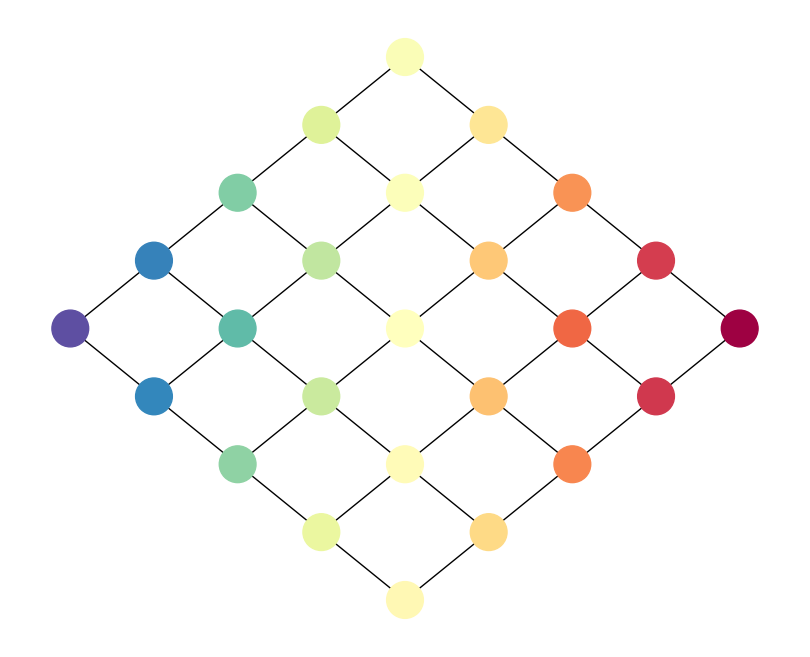
\includegraphics[width=0.5\linewidth]{figures/background/grid_eigenvector.png}
    \caption{The $\lambda_{2}$-eigenvector for a grid, also called the Fiedler Vector of the grid.}
    \label{fig:placeholder}
\end{figure}

We now introduce the most common signal model used in the graph signal processing literature, the bandlimited signal model. A $k$-\emph{bandlimited signal} is a linear combination of the first $k$ columns of $\matr{U}$\cite{EOptimalChen}. It is also called a $\lambda_{k}$-bandlimited signal, where $\lambda_{k}$ is the $k^{th}$ eigenvalue of the graph shift operator \cite{shomorony2014sampling}. To construct these signals, we define $\projbl$ as the projection operator that $k$-bandlimits a signal:
\begin{equation} 
    \projbl = \matrsubU{N}\matrsubU{N}^{T}.
\end{equation}
%To facilitate our discussion we first introduce a few handy notations.

%Sec II.B

%We can understand $\projbl$ as converting a signal into the nearest $k$-bandlimited signal.  %, and the space of such signals is called a Paley-Wiener space \cite{pesenson2008sampling}.%, written either as $PW_{\omega}(\mathcal{G})$ for any $\omega \in [\lambda_{k}, \lambda_{k+1})$ or $\text{BL}_{k}(\matr{U}^{T})$ \cite{EOptimalChen}.

It is rare for observed signals to be perfectly bandlimited{\color{black}. While this can be modelled by assuming the underlying signal to be reconstructed is not bandlimited but rather} `approximately bandlimited signals'\cite{chen2016signal, lin2019active}, or from other more general priors \cite{tanaka2020generalized, hara2022sampling}, in this thesis we take the more common approach \cite{wang2018optimal, wang2019low,bai2020fast, puy2018random, tremblay2017determinantal} of assuming {\color{black}the underlying signal is $k$-bandlimited} with additive observation noise. %We assume we observe a corrupted signal $\vect{y} = \vect{x} + \vect{n}$ %at a subset of the vertices $\set{S}$ 

We now discuss quantification of noise. In the literature, noise levels are often described using the SNR = $\frac{\expect{\sqnormvec{ \vect{x} }}}{\expect{\sqnormvec{\vect{n}}}}$, a ratio of norms which must be positive. It is common in the literature to express the SNR in decibels, which may be negative, while its ratio form remains positive. We will use the ratio form unless otherwise noted, so for example $-20dB$ will be written as $10^{-20/10}  > 0$.

\subsubsection{Graph Filtering}
In our section on signal models, we developed a notion of `bandlimiting', which is parallel to the DSP notion of bandlimiting. We briefly make this parallel more explicit by talking about graph filters, before going on to discuss missing data.

A fundamental operation in signal processing is filtering, which operates on the frequencies of the signals. Approaches to generalising DSP generally maintain the convolution theorem -- that convolution in the original domain is (pointwise) multiplication in the frequency domain (for a comparison of the generalisation of the DFT to groups via Pontryagin Duality and the generalisation to graphs we discuss here, see \cite{ji2023faces}). GSP uses the convolution theorem and the graph Fourier transform to generalises filtering to graph filtering.

We spell this generalisation out explicitly. A graph filter $h: \mathbb{R} \to \mathbb{R}$ is applied by computing the Fourier transform, applying $h$ in the frequency domain, and then applying the inverse Fourier transform.
\begin{equation}
    \vect{x}_{filtered} = \matr{U}\text{diag}(h(\lambda_{1}),\ldots,h(\lambda_{N}))\matr{U}^{T}\vect{x}.
\end{equation}

If $h(\lambda) = \mathds{1}\{
\lambda \leq \lambda_{k} \}$ (known as a bandpass filter) then the corresponding filtering operation is applying $\projbl$.

If the filter is a polynomial $p$, then the filtering operation can be written as directly applying the polynomial of the shift operator to the signal. For example, if the shift operator is $\matr{L}$ and if $p(x) = x^{2} + x + 1$ then $x_{filtered} = (\matr{L}^{2} + \matr{L} + \matr{I})\vect{x}$, thus polynomial filters can be applied without spectral decomposition, making such filters much more computationally efficient.


\subsection{Graph Machine Learning}
Graph Machine Learning (GML) is a field extends machine learning techniques by incorporating graph information. It focuses on Graph Neural Networks (GNN), architectures based on neural networks which can be applied to graph-structured data.
\subsubsection{Graph Neural Networks} \label{sec:GNN_background}
GNNs can be viewed from a spatial or spectral perspective. In the spatial perspective, in each layer data is aggregated via message passing \cite[Section 5.3]{bronstein2021geometric}, while in the spectral perspective GNNs are constructed using graph filters as building blocks \cite{gama2018convolutional}. There is an equivalence between graph convolutions constructed by these two methods \cite{balcilar2020bridging}.

We now briefly cover the Graph Convolutional Network (GCN) architecture, one of the original GNNs, and Simplified Graph Convolutions (SGCs), a linearisation of the GCN.

GCNs adapt feedforward neural networks by convolving the 
GCN using the normalised adjacency matrix \cite{kipf2016semi}. The following equation expresses the relationship between layers:
\begin{equation}
    \matr{X}_{l} = \sigma(\tilde{\matr{A}}\matr{X}_{l-1}\matr{W}_{l-1})
\end{equation}
where $\matr{X}_{0}$ is the initial feature matrix provided $\matr{W}_{i}$ are learnable weight matrices, $\matr{X}_{i}$ is the output of layer $i$ and $\sigma$ is a nonlinearity like ReLU. As $\tilde{\matr{A}} = \matr{I} = \tilde{\matr{L}}$, each layer without the nonlinearity can be viewed as a low-pass graph filter with shift operator $\tilde{\matr{L}}$ followed by a learnable linear feature update. It is also common to use the augmented adjacency matrix with $\gamma=1$, $\tilde{\matr{A}}_{1}$.

The Simplified Graph Convolution (SGC) architecture has the following per-layer equation, which removes the nonlinearity from the GCN formulation:
\begin{equation}
    \matr{X}_{l} = (\tilde{\matr{A}}\matr{X}_{l-1}\matr{W}_{l-1}).
\end{equation}
Equivalently, for the SGC one can write:
\begin{equation}
    \matr{X}_{l} = \tilde{\matr{A}}^{l}\matr{X}_{0}\prod_{i=0}^{l-1}\matr{W}_{i}).
\end{equation}
Writing $\tilde{\matr{A}} = \matr{I} - \tilde{\matr{L}}$, this can be seen as a low-pass graph filter with the normalized Laplacian as a graph shift operator, coupled with a linear feature update.

\section{Problem Formulation}
\label{sec:thesis_define_MMSE}
We now write down our general setting in order to formulate the goals of the thesis mathematically. In each chapter, we will specialise the setting explicitly. 

Throughout this thesis we assume we have:
\begin{itemize}
    \item A known graph $\mathcal{G}$ which is connected and undirected;
    \item A random `feature matrix' $\matr{X}\in\mathbb{R}^{N \times d}$, where each column is a smooth graph signal and we know their joint distribution;
    \item Random observation noise $\vect{n}$, which has the same shape as $\matr{X}$ and known distribution
    \item Observations of $\matr{X}$ at a sample set $\set{S}$ corrupted by the noise $\vect{n}$ (i.e., $\msubgen[\set{S},\set{D}]{\matr{X} + \vect{n}}$);
    \item A linear reconstruction $\hat{\matr{X}}$ from these observations, (i.e., $\hat{\matr{X}} = \matr{R}_{\set{S}} \msubgen[\set{S},\set{D}]{\matr{X} + \vect{n}}$).
\end{itemize}
In Chapters \ref{ch:proj1_LS} \& \ref{ch:proj1_GLR} $\matr{X}$ has a single column and we refer to it as the graph signal $\vect{x}$ (and similarly we refer to $\hat{\matr{X}}$ as $\hat{\vect{x}}$). 
In Chapter \ref{ch:proj2} we  introduce the downstream task of binary classification, and also need:
\begin{itemize}
    \item Binary labels $\matr{l} \in \{-1,1\}^{N}$ generated by a known function $f:\, \mathbb{R}^{N \times d}\to \mathbb{R}^{N}$  (i.e., $\vect{l} = \text{sign}\left(f\left(\matr{X}\right)\right)$ with sign elementwise).
\end{itemize}
We consider the following losses:
\begin{align}
    &\text{MMSE} &&= \expect[\matr{X}, \vect{n}]{||{\vect{X} - \hat{\vect{X}}}||^{2}_{F}},\\
    &{\text{Classification Loss}} &&= {\sum_{i \in \set{V}}\prob{\text{sign}\left(f(\matr{X})_{i}\right) \neq \text{sign}(f(\hat{\matr{X}})_{i})}}.
\end{align}
We also refer to MMSE as the reconstruction loss when it is unambiguous. 

In this thesis, we seek to address the following two questions. As noise levels, sample selection methods and reconstruction methods vary:
\begin{enumerate}
    \item How does MMSE vary with sample size?
    %\item How does Classification Loss relate to MMSE?
    \item How does Classification loss vary with sample size, and how does this relate to MMSE?
\end{enumerate}

\section{Literature Review}
\label{sec:thesis_lit_review}
%We review the literature on incomplete information on graphs in GSP and GML. We focus on sample set selection

%The GSP literature frames
\subsection{The Impact of Sample Size on Missing Data}
%\subsubsection{Sampling for Reconstruction}
We now survey the literature on incomplete information. We begin with a survey of the GSP literature, with an eye to the impact of sample size. GSP approaches incomplete information by generalising the theory of sampling and reconstruction from signal processing. We begin with reconstruction of the missing data, and then move on to sampling.

\subsubsection{Reconstruction Methods}
There are many reasons data may be missing -- because it has come from polling or sampling, because it was deleted adversarially or for other reasons, like data corruption. In this thesis, we focus on the approach of reconstructing data to handle missing data, which also known as inpainting. We begin with an intuitive example.

Consider our social network example, with our graph signal being the ages of each person. We have assumed people have similar ages to their friends (the smoothness assumption). If we don't know the age of a person, but we do know all of their friends are 25, then it is a reasonable assumption to assume they are 25. This idea can be viewed as fitting a bandlimited signal (the true, unobserved data -- in the given example, we are fitting the constant signal, which is the $\lambda_{1}$ eigenvector of $\matr{L}$) or as maximising some smoothness functional conditional on the resultant signal matching observed data. These two approaches yield different methods of inpainting data in more complex situations, which we present below.

We define a \emph{reconstruction method} (or `interpolation operator' \cite{chamon2017greedy}) to take potentially noisy observations on a vertex sample set $\set{S}$ and reconstruct the signal across all vertices. In this paper we focus on LS and GLR, and we present their objectives here:
\begin{flalign}
        &\text{LS:} \hspace{0.13\columnwidth}  \hat{\vect{x}} =  \argmin_{\vect{x} \in \text{span}(\matrsubU{N})} || \vectsub[S]{x} - \vect{y} ||_{2}   & \label{eq:LS_Defn} \\ 
        &\text{GLR:} \hspace{0.1\columnwidth}  \hat{\vect{x}} = \hspace{11pt} \argmin_{\vect{x} \in \mathbb{R}^{N}}  \sqnormvec{ \vectsub[S]{x} - \vect{y}} + \mu \vect{x}^{T}\matr{L}\vect{x} & \label{eq:GLR_Defn}
\end{flalign}
GLR can be seen to be a form of Tikhonov regularisation \cite{belkin2004tikhonov}.
We summarise their differences in Table \ref{tab:tbl1}, labelling the input parameters into the reconstruction, whether they are biased and whether they require computation of the {\color{black}eigenbasis} $\matrsubU{N}$. 


\begin{table}[h]
\caption{The LS and GLR reconstruction Methods.}
\renewcommand*{\arraystretch}{1.5}
\centering
\begin{tabular*}{\textwidth}{l@{\extracolsep{\fill}}ccc}
    %\begin{tabular}{lccc}
    \toprule
      & \textbf{Parameters} & \textbf{Biased} & \textbf{Requires Computing $\matrsubU{N}$} \\
    \midrule
        LS  & $k$ & $\times$ & $\checkmark$ \\
        GLR  & $\mu$ & $\checkmark$ & $\times$ \\
    \bottomrule
    \end{tabular*}
\label{tab:tbl1}
\end{table}

Our analysis of LS also applies to the commonly used iterative reconstruction method, Projection onto Convex Sets \cite{narang2013localized}, as POCS converges to LS.

We call a reconstruction method \emph{linear} if it is linear in its observations. For a fixed vertex sample set $\set{S}$ we can represent a linear reconstruction method by a matrix $\matr{R}_{\set{S}} \in \mathbb{R}^{N \times |\set{S}|}$.

\begin{remark}
    LS and GLR are both linear:
    \begin{align}
    \textrm{LS:\quad} \matr{R}_{\set{S}} &= \matrsubU{N}\matrsubU{S}^{\dagger} \label{eq:defn_RS:LS}\\
    \textrm{GLR:\quad} \matr{R}_{\set{S}} &= \msub[N,S]{( \proj{S} + \mu \matr{L})^{-1}} \label{eq:defn_RS:GLR}
    \end{align}
\end{remark}
\noindent where for a matrix $\matr{A}$, $\matr{A}^{\dagger}$ is its Moore-Penrose pseudoinverse.

Across all linear models under the noisy setting, LS leads to the minimum-variance unbiased estimator of $\vect{x}$ \cite{gauss1823theoria} {\color{black} for $k$-bandlimited signals and full-band noise}, which theoretically justifies us focusing our analysis on LS. 
On the other hand, GLR implicitly assumes a multivariate Gaussian signal with covariance $\matr{L}^{\dagger}$\cite{dong2016learning}, which is slightly mismatched with the $k$-bandlimited signal model we focus on in this paper. Nevertheless, in practice GLR is still often used for large graphs as computing $\matrsubU{N}$ for LS is slow \cite{puy2018random, bai2020fast}. It is also a typical regression model that promotes signal smoothness and has been widely adopted in the literature \cite{belkin2004semi}. Because of these considerations we believe GLR is still a meaningful case to study.

Finally, we clarify what we mean when we consider LS with sample size less than bandwidth. {\color{black} In this case }if LS is defined as the minimisation of the objective \bs{(\ref{eq:LS_Defn})} there are multiple solutions. Thus, we follow \cite{anis2016efficient} and define the LS reconstruction as the 
unique minimum-norm solution \cite[Sect. 5.5.1]{golub13}, hence (\ref{eq:defn_RS:LS}) applies regardless of sample size. 


We now briefly discuss variants of the two reconstruction methods above. GLR is widely considered a `regularised' method and less sensitive to noise, and LS is an unregularised method. Feature Propagation  \cite{rossi2021unreasonable} (FP) can be viewed as taking the limit of $\mu \to 0$ in GLR, giving an unregularised counterpart of GLR which does not smooth the already observed data. We provide an exact mathematical statement characterising this statement, along with a proof, in Appendix \ref{app:Feature_Propagation_limit_is_GLR}. We define the corresponding $\matr{R}_{\set{S}}$ for FP:
    \begin{align}
    \textrm{FP:\quad} \matr{R}_{\set{S}} &= \matrsub[N,S]{I} + \msubgen[\set{N},\set{S}^{C}]{\matr{I}}\msubgen[\set{S}^{C}]{\matr{L}}^{-1}\msubgen[\set{S}^{C},\set{S}]{\matr{L}}.\label{eq:defn_RS:FP}
    \end{align}
On the other hand, if the graph signal $\vect{x}$ and observation error $\vect{n}$ are multivariate gaussians with known mean and covariance, then we can use the expectation of $\vect{x}$ conditional on the observations we have made as a reconstruction of $\vect{x}$. Under a bandlimited signal model, this is a regularised version of LS which requires exact knowledge of the noise level, and is called `Optimal Bayesian Reconstruction' \cite{chamon2017greedy}. In this thesis we do not attempt to characterise this or other noise-adaptive methods; we assume that $\matr{R}_{\set{S}}$ is not dependent on $\sigma$.
% It has been proven in this case that decreasing sample size must increase MSE \cite{chamon2017greedy}. We do not attempt 

\subsubsection{Sampling \& Optimal Design of Experiments}
Sampling is the process of acquiring partial data. When trying to generalise sampling from classical signal processing to the graph setting, two issues arise \cite{tanaka2020sampling} -- defining graph frequencies, which we have addressed above, and generalising periodic sampling. Periodic sampling is difficult to generalise spatially, because of the irregularity of graph structure prohibits an easy definition of `periodic' except on very specific graph structures (such as the ring graph), and the shift operators traditionally chosen in GSP make defining periodic sampling via shift-invariance difficult. Instead, GSP approaches vertex sample selection much more directly. We now think about vertex sample selection from the ground up.

To meaningfully contrast choices of vertex sample set size and selection, we need to evaluate reconstruction performance, and we do so by certain optimality criteria. In the case of a noiseless $k$-bandlimited signal, the main optimality criterion for a vertex sample set $\set{S}$ is whether it is a \emph{uniqueness set} 
 \cite{pesenson2008sampling}, that is, if we can perfectly reconstruct any $k$-bandlimited signal observed on $\set{S}$. Such a set always exists and $\set{S}$ is a uniqueness set for a bandwidth $k$ if and only if $\text{rank}(\matrsubU{S}) = k$ \cite{anis2016efficient}. 
 
 In the case of additive observation noise, there are multiple common optimality criteria \cite[Chapter 6]{pukelsheim2006optimal}:

\begin{itemize}
    \item \emph{MMSE criterion}: Minimise  average MSE. \cite{wang2018optimal,wang2019low, mfn}
    \item \emph{Confidence Ellipsoid criterion}: Minimise the confidence ellipsoid around the eigenbasis co-efficients. \cite{jayawant2021doptimal, tremblay2017determinantal, mfn}
    \item \emph{WMSE criterion}: Minimise worst-case MSE. \cite{bai2020fast, EOptimalChen}
\end{itemize}

\noindent 
Under LS, these criteria have the following names and forms:
\begin{align}
    \text{\emph{(MMSE)} A-Optimality:} &\text{ minimise } \text{tr}(\matr{P}^{-1}) \label{eq:A-optimality}\\
    \text{\emph{(Conf. Ellips.)} D-Optimality:} &\text{ maximise } \text{det}(\matr{P})
 \label{eq:D-optimality}\\
    \text{\emph{(WMSE)} E-Optimality:} &\text{ maximise }
        \lambda_{min}(\matr{P}) \label{eq:E-optimality}
\end{align}
%\noindent where $\matr{P}$ is defined as %where $\lambda_{min}(\matr{P})$ is the minimum eigenvalue of $\matr{P}$ defined as: %\in \mathbb{R}^{d \times d}$,
\begin{flalign}
    &\text{where }&\matr{P} = \begin{cases}
        \projbl[S] &\text{if }|\set{S}| < k \\
        \matrsubU{S}^{T}\matrsubU{S} &\text{if }|\set{S}| \geq k
    \end{cases} \qquad\qquad\qquad&
\end{flalign}  

\noindent and we define $\trace{\matr{P}^{-1}} = +\infty$ in (\ref{eq:A-optimality}) if $\matr{P}$ is not invertible.

Pukelsheim derives A-, D- and E-Optimality criteria from the theory of matrix means. Pukelshiem also notes that matrix mean theory also implies T-Optimality, maximising $\text{tr}(\matr{P})$, which has been employed approximately in the GSP setting in \cite{puy2018random}. However, this optimality criterion does not translate to a natural objective in the way we have described above for A-, D- and E-Optimality -- Pukelsheim describes T-Optimality as `rather meaningless'\cite[Section 6.5]{pukelsheim2006optimal} and lists ways in which its `weakness' causes a list of `pathologies', making discussion of the theory of sampling more difficult with little gain. Therefore, we exclude T-Optimality from our theoretical analysis. 

We note that if $\matr{P}$ is invertible, then we have the following relationships between these criteria:
\begin{align}
    \lambda_{min}(\matr{P})^{-1} &< \text{tr}(\matr{P}^{-1}) \leq N \lambda_{min}(\matr{P})^{-1} \\
    \lambda_{min}(\matr{P})^{N} &< \text{det}(\matr{P}) \\
    N \cdot \text{det}(\matr{P})^{-\frac{1}{N}} &\leq \text{tr}(\matr{P}^{-1})
\end{align}
where the first two inequalities are immediate from writing out trace and det in terms of eigenvalues, and the last inequality arises from the AM-GM inequality applied to the reciprocal of the eigenvalues of $\matr{P}$. These inequalities mean that optimising one of the three presented criteria means that we are simultaneously optimising a bound for the other two criteria.

\subsubsection{GSP Literature on Sample Size}
In the GSP literature, the vast majority of studies on graph-based sampling focus on designing efficient sampling schemes that are approximately optimal under the criteria listed above \cite[Chapter 6]{pukelsheim2006optimal}, because optimal vertex choice under noise is in general NP-hard \cite{nikolov2022proportional} and greedy sampling is provably effective \cite{chamon2017greedy}. While these studies provide useful understanding in terms of sampling and reconstruction for graph signals, they focus on the performance of sampling schemes at fixed sample sizes \cite{xie2019bayesian, puy2018random,shomorony2014sampling, tremblay2017determinantal,wang2018optimal,wang2019low, bai2020fast,  anis2016efficient}, while much less attention has been paid to understanding the impact of varying sample size on the mean squared error (MSE) of reconstruction. Sample size is an important parameter in both understanding and using sampling schemes, especially in the common setting of a fixed sample budget. %across all possible levels of noise, which is important for the application of graph sampling to domains such as finance \cite{nabar2023conservative} where the noise may be greater than the signal and domains where observing more samples might not be feasible and subsampling is more feasible.

\begin{table}[ht]
    \centering
    \caption{Studies on the Impact of Sample Size on MSE}
    \begin{subtable}[h]{\linewidth}
        \centering
        \begin{tabularx}{\linewidth}{lp{2cm}Xp{4cm}}
            \toprule
            \textbf{Reference} & \textbf{Considers Noise?} & \textbf{Reconstruction Method} & \textbf{Range of Possible Sample Sizes} \\
            \midrule
            Tremblay, 2017 \cite{tremblay2017determinantal} & \checkmark & LS, GLR & Limited \\
            Wang, 2018 \cite{wang2018optimal} & \checkmark & LS & Limited \\
            Wang, 2019 \cite{wang2019low} & \checkmark & LS & Limited \\
            Bai, 2020 \cite{bai2020fast} & \checkmark & GLR & Limited \\
            Anis, 2016 \cite{anis2016efficient} & \checkmark & LS & Full \\
            \bottomrule
        \end{tabularx}
        \caption{Empirical Results}
    \end{subtable}
    
    \vspace{1em}
    
    \begin{subtable}[h]{\linewidth}
        \centering
        \begin{tabularx}{\linewidth}{lp{2cm}Xp{4cm}}
            \toprule
            \textbf{Reference} & \textbf{Considers Noise?} & \textbf{Reconstruction Method} & \textbf{Range of Possible Sample Sizes} \\
            \midrule
            Puy, 2018 \cite{puy2018random} & \checkmark & LS & Limited \\
            Chamon, 2017 \cite{chamon2017greedy} & \checkmark & LS (Regularised) & Full \\
            Shomorony, 2014 \cite{shomorony2014sampling} & \texttimes & LS & Full \\
            Belkin, 2004 \cite{belkin2004tikhonov} & \texttimes & GLR (Variant) & Full \\
            \textbf{Chapter \ref{ch:proj1_LS}} & \textbf{\checkmark} & \textbf{LS} & \textbf{Full} \\
            \textbf{Chapter \ref{ch:proj1_GLR}} & \textbf{\checkmark} & \textbf{GLR} & \textbf{Full} \\
            \bottomrule
        \end{tabularx}
        \caption{Theoretical Results}
    \end{subtable}
    \label{tbl:Lit_review}
\end{table}

The literature studies the impact of sample size both empirically and theoretically \bs{(summarised in Table \ref{tbl:Lit_review})}, and can be further divided by the setting considered: whether the observations are noisy or noiseless, and by which reconstruction method. 

\paragraph{Empirical results} Empirical results, linked to sampling schemes, are usually obtained in the noisy setting under least squares (LS) reconstruction or its variants \cite{ tremblay2017determinantal,wang2018optimal,wang2019low,chamon2017greedy} or graph-Laplacian regularised (GLR) reconstruction \cite{bai2020fast, tremblay2017determinantal}. These results show that MSE decreases as sample size increases in a restricted range of noise level and sample size. An exception is \cite[Fig. 1]{anis2016efficient} which empirically shows non-monotonicity of MSE with sample size under LS as it considers the {\color{black}full range of possible sample sizes, including sample sizes less than bandwidth,} and a relatively high noise level. 

\paragraph{Theoretical results -- LS} We now survey the theoretical results around reconstruction error in the literature. In order to prove these results, they each make changes to the setup found in the empirical results cited either in the signal model, the reconstruction method or the sampling method. We begin by discussing the results on LS reconstruction and variants of LS reconstruction. Firstly, Shomorony et al. \cite{shomorony2014sampling}  assume a noiseless bandlimited signal model ($\vect{n} = 0$). They show that for any graph, there is a sample set of size $k$ which allows for perfect reconstruction of any noiseless $k$-bandlimited signal by LS reconstruction (i.e. a uniqueness set of size $k$ for $k$-bandlimited signals always exists). Their approach relies on the signal living in a subspace of dimension $k$, and so does not immediately extend to cases where the signal is peturbed, for example by noise. Chamon et al. \cite{chamon2017greedy} address reconstruction in the case of $k$-bandlimited signals; they prove for a variant of LS, Optimal Bayesian Reconstruction, that MSE decreases as sample size increases in the noisy setting and provide bounds on the impact of sample size on MSE. Their reconstruction method is defined as minimising covariance across all reconstruction methods, including ones which ignore subsets of the nodes \cite[(7)]{chamon2017greedy}, and this is essential to their proofs; thus their statements around the monotonicity of MSE with sample size are restricted to this specific optimal form of regularised LS which requires knowledge of noise, and do not necessarily carry over to the setting of unregularised LS reconstruction (or GLR reconstruction). 

Finally, we discuss theoretical results restricting sample set selection. We discuss two results. Firstly, Puy et al. \cite[Theorem 6]{puy2018random} assume unregularised LS and noisy reconstruction, but require random sampling where each node is chosen with non-zero probability. Puy et al. use results from concentration of measure to prove an MSE upper bound that is tight and decreasing in sample size; however, this result is practically constrained to the case where sample size is greater than or equal to bandwidth \cite[(3)]{puy2018random}. Secondly, Tremblay \cite{tremblay2024graph} exploits relationships between the MMSE criteria $\text{tr}(\matr{P}^{-1})$ itself and the probability of sampling $\matr{P}$, which we outline. Consider the fact that under uniform random sampling of $\set{S}$, $\expect[\set{S}]{\text{tr}(\matrsub[S]{X})} = \frac{m}{N}\text{tr}(\matr{X})$ is easy to calculate, and remains the same under a change of basis; $\expect[\set{S}]{\text{tr}\left(\msubgen[\set{S}]{\matr{U}\matr{X}\matr{U}^{T}}\right)} = \frac{m}{N}\text{tr}(\matr{X})$ for any change of basis $\matr{U}$. This is because the trace is preserved under a change of basis. This notion can be generalised through results on the exterior algebra; firstly, the sum of the determinants of principal submatrices, called principal minors, is invariant to changes in basis and can be calculated from the eigenvalues of the overall matrix \cite[Theorem 1.2.16]{horn-and-johnson}. This can be seen as a generalisation of the trace as the trace is the sum of the determinants of the 1 \texttimes 1 principal submatrices. Secondly, for an $m \times m$ matrix $\matr{P}$, $\text{tr}(\matr{P}^{-1})\text{det}(\matr{P}) = \text{tr}(\matr{P}^{-1}\text{det}(\matr{P})) = \text{tr}(\text{adj}(\matr{P}))$, the trace of the adjugate of $\matr{P}$, which is the sum of the $m-1$ principal minors of $\matr{P}$. Combining these facts allows for calculation of the expected MSE, which we know can be written as $\expect[\set{S}]{\text{tr}(\matr{P}^{-1})}$ (see \ref{eq:A-optimality}), when sample set selection is  done randomly with probability proportional to the determinant of the submatrix. This is called determinental sampling, and is studied by Tremblay \cite{tremblay2024graph}. Typically, determinental sampling does not provide a fixed sample size, instead sampling over all possible sample sizes proportional to said determinant, and Tremblay provides a bound \cite[(4.14)]{tremblay2024graph} on the MMSE under said scheme without fixed sample size; however, he also defines fixed-sample size determinental sampling schemes, and links to results in the wider literature which immediately give MSE bounds for such fixed size schemes as sample size varies \cite[Theorem 4]{derezinski2017unbiased}. These bounds, however, would only apply to fixed-size determinental sampling.

\paragraph{Theoretical results -- GLR}We now discuss the GLR reconstruction setting. Theoretical work on GLR reconstruction is scarce in the GSP literature; GLR is generally considered in noisy scenarios as the implicit signal model of GLR is a multivariate gaussian signal with covariance $\matr{L}^{\dagger}$ \cite{dong2016learning}, which does not match with the usual bandlimited signal model.  To construct an Optimal Bayesian Reconstruction variant of GLR would potentially involve studying LapRLS \cite[Section 4.2]{belkin2006manifold}, and studies on LapRLS are scarce in the GSP literature; Finally, GLR reconstruction does not immediately lend itself to being structured in the form $\text{tr}(\matr{P})$, making analysis under determinental sampling much less immediate.

In the Learning Theory literature, Belkin et al. \cite{belkin2004tikhonov} study a variant of GLR reconstruction which only provides reconstructions where the reconstructed graph signal $\vect{x}$ must have the property $\vect{1}^{T}\vect{x}=  0$; they make this assumption for stability reasons. They provide a theoretical bound on the generalised learning risk of a variant of GLR reconstruction as sample size varies which only reconstructs signals where the sum of the graph signal values are 0; they make this assumption for stability reasons. They conduct analysis via a Reproducing Kernel Hilbert Space approach, viewing GLR as a variant of Tikhonov regularisation and the Laplacian as providing an inner product. The result they prove is very general, requiring only a boundedness constraint on the signal model; however, it is difficult to understand their results in terms of MMSE, and their results do not apply to unconstrained version of GLR. In general, theoretical quantification of the properties of reconstruction error as sample size varies for unconstrained GLR has not been tackled by the GSP community.

While these theoretical results provide valuable insight, the settings they are based on do not always agree with those in the empirical studies above, hence a generic understanding is still lacking. %The fourth theoretical result by Puy et al. \cite[Theorem 6]{puy2018random} assumes unregularised LS and noisy reconstruction, and proves an MSE upper bound that is tight and decreasing in sample size; however, this result is practically constrained to the case where sample size is greater than or equal to bandwidth \cite[Eq. 3]{puy2018random}.
%can give insight to the impact of MSE, as they are in a different setting to the empirical results they do not apply in that setting.

%In this chapter, we fill the gap in the literature by providing a theoretical characterisation of the impact of sample size on \bs{the average} MSE \bs{ (or MMSE  -- see Section \ref{sec:Optimality_Criteria})} across the full range of possible sample sizes in the most common settings, i.e. noisy observations and LS or GLR reconstruction. More specifically, we focus on whether under sufficiently low SNRs, decreasing sample size may actually decrease MSE. Furthermore, we investigate both the full range of sample sizes and all possible levels of noise, which is important for the application of graph sampling to domains where the noise may be greater than the signal \xd{(e.g. finance, with typically low signal-to-noise ratio \cite{nabar2023conservative}, or environmental sciences,  with inaccurate measurements from low-cost sensors \cite{bush2023impact})} or when observing more samples might not be feasible (e.g. resource-constrained settings). This breadth is only possible through our rigorous theoretical characterisation which allows us to understand behaviour at high noise levels\bs{,} to characterise behaviour on arbitrarily large graphs\bs{,} and to show when certain behaviours of MSE happen and why. %While theorems often need to be narrow in scope to allow for tractable proofs, our results are notable in how loose their restrictions are; our results for LS reconstruction apply to all graphs and every determinstic sampling scheme in the literature, while the conditions of our main result for GLR reconstruction under full-band noise, empirically, hold for every Erdős–Rényi, Stochastic Blockmodel and Barabasi-Albert graph tested (Table \ref{tbl:empirical_probabilities_conditions}).

\subsection{The Impact of Downstream Tasks on Missing Data}
The theoretical results in the GSP literature have been derived under reconstruction loss, and so do not immediately carry over to other tasks such as classification, as they rely on the specific structure of reconstruction loss -- for example, the proof of near-optimality of greedy sampling on graphs \cite{chamon2016near} relies on the loss's (approximate) supermodularity. Thus, there is a significant lack of investigation in the GSP literature of the impact of incomplete data on downstream learning tasks. One notable exception is Gama et al. \cite{gama2020rethinking}, who look at optimising reconstruction and sampling in the light of a known linear downstream task; however, their results focus on the design of a sample scheme tightly coupled to a `sketching operator' which is specific to the linear downstream task. Use of a non-standard reconstruction method means it is difficult to interpret the relationship between reconstruction error and task error, and they do not explicitly examine the relationship between task performance and sample size. We also note that the results of Chamon et al \cite{chamon2017greedy} allow for a linear transform in a manner similar to Gama et al., however there is little discussion on the impact of the transform.

The graph machine learning (GML) community, on the other hand, does address the issue of incomplete data in the context of downstream tasks such as node classification. They take two main approaches -- label prediction and feature imputation. Label prediction sidesteps the issue of missing data by directly predicting the missing node class labels. Examples of label prediction include label propagation \cite{zhu2003semi}, which can be seen as a generalised form of feature propagation \cite{belkin2004tikhonov}, or by using graph neural networks (GNNs) on the partial data with modified message passing \cite{jiang2020incomplete, chen2020learning}. Feature imputation involves reconstructing the graph signals, potentially alongside missing edges, usually as a pre-processing step to inference. Such methods include matrix completion methods like Kalofolias et al. \cite{kalofolias2014matrix} who minimise a graph-smoothness regularised version of the nuclear norm, and autoencoder-based methods such as Spinelli et al\cite{spinelli2020missing} who build on Generative Adversarial Networks (GANs). Another example is Rossi et al.'s Feature Propagation \cite{rossi2021unreasonable}, which is a graph Laplacian-based feature imputation method that applies a GSP-motivated approach to downstream tasks such as classification with GNNs. Finally, some approaches combine label prediction and feature imputation in an end-to-end training framework  such as Taguchi et al.'s GCNMF which implicitly models the missing data with a Gaussian  Mixture Model\cite{taguchi2021graph}, or You et al. \cite{you2020handling} whose GRAPE transforms the dataset into a bipartite graph between nodes with known features and unknown features; they use this to transform the missing data and label imputation problem into an edge and node-label prediction task respectively, and use graph learning techniques from these fields. While work in GML engages with missing data in settings with varied downstream tasks, it has done so through an empirical lens -- evaluating the performance of the proposed methods on specific datasets -- and thus theoretical results remain scarce.